\begin{figure}[tp]
 \centering
 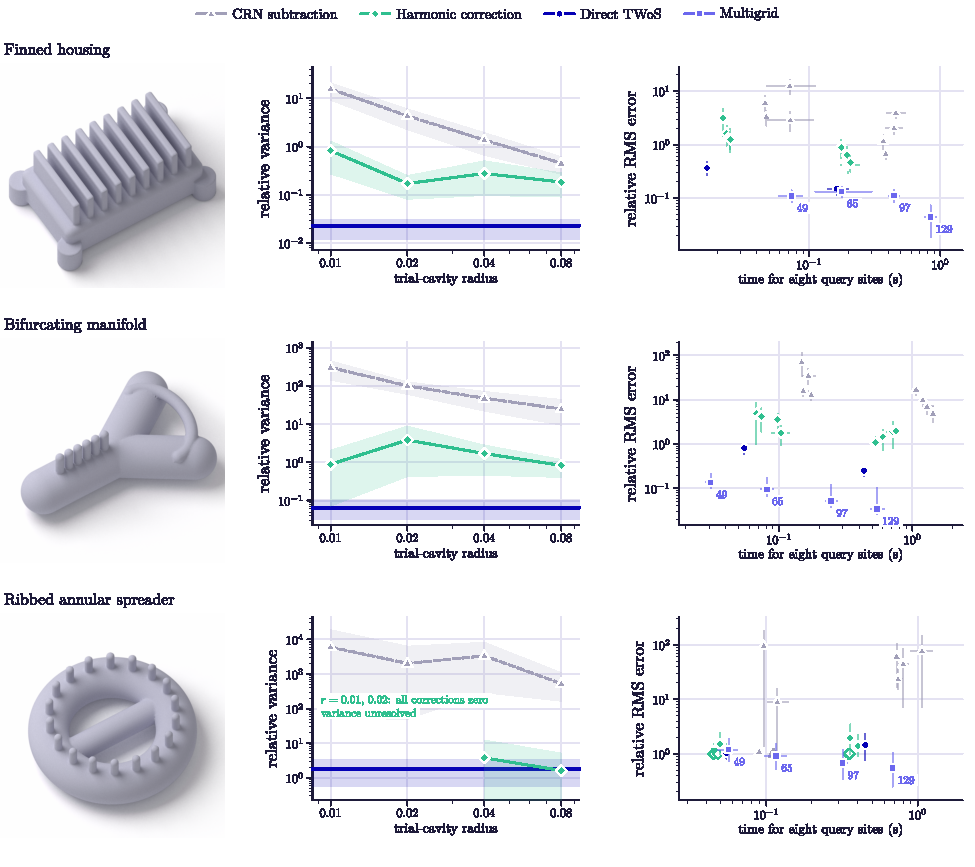
\includegraphics[width=\textwidth]{figures/submission-estimators.pdf}
 \caption{\textbf{Actual-geometry estimator comparisons.}
 Each row uses eight fixed, protected query sites on one mesh.
 The center plots normalize summed site variances by the squared norm of the
 high-budget reference and use 2,048 paths per site. Bands give pointwise 95\%
 bootstrap intervals from sixteen independent repeat vectors and sixteen
 independent reference batches. Direct TWoS has no trial-radius input;
 its horizontal band is repeated for comparison, not independently remeasured
 at every radius. Right: relative RMS error and wall time at both Monte Carlo
 budgets and all finite radii, with four deterministic grid resolutions labeled.
 Bars reflect repetition and reference-sampling uncertainty; deterministic
 grid error bars reflect only reference sampling, while their runtime bars
 use five repeated solves. Finite-radius, discretization,
 and termination biases are not enclosed. The reference is an independent,
 high-budget TWoS estimate, not exact ground truth. All-zero correction settings
 are marked unresolved and use open error--cost markers; their collapsed bootstrap intervals are suppressed.}
 \label{eg:submissionestimators}\label{fig:submissionestimators}
\end{figure}
